  {\large \fontB Description:}
  
  {\bf solG} is a 2-dimensional analytical solution to the Cauchy equations with the acceleration term set to zero
  to represent creeping flow. The boundary conditions are free-slip everywhere on a unit domain. 
  The viscosity is layered with a jump at $ z=z_c $.
  The flow is driven by a dense block.
  \\

  {\large \fontB Parameters:}
 
  The variable parameters of this solution are:
  \begin{itemize}
    \item{density parameter: $ \sigma $.}
    \item{viscosities: $\eta_A$ and $\eta_B$.}
    \item{width of dense block: $dx$.}
    \item{centre of dense block: $x_0$.}
    \item{bottom of dense block: $z_c$.}
    \end{itemize}

  \begin{SCfigure}[][h]
    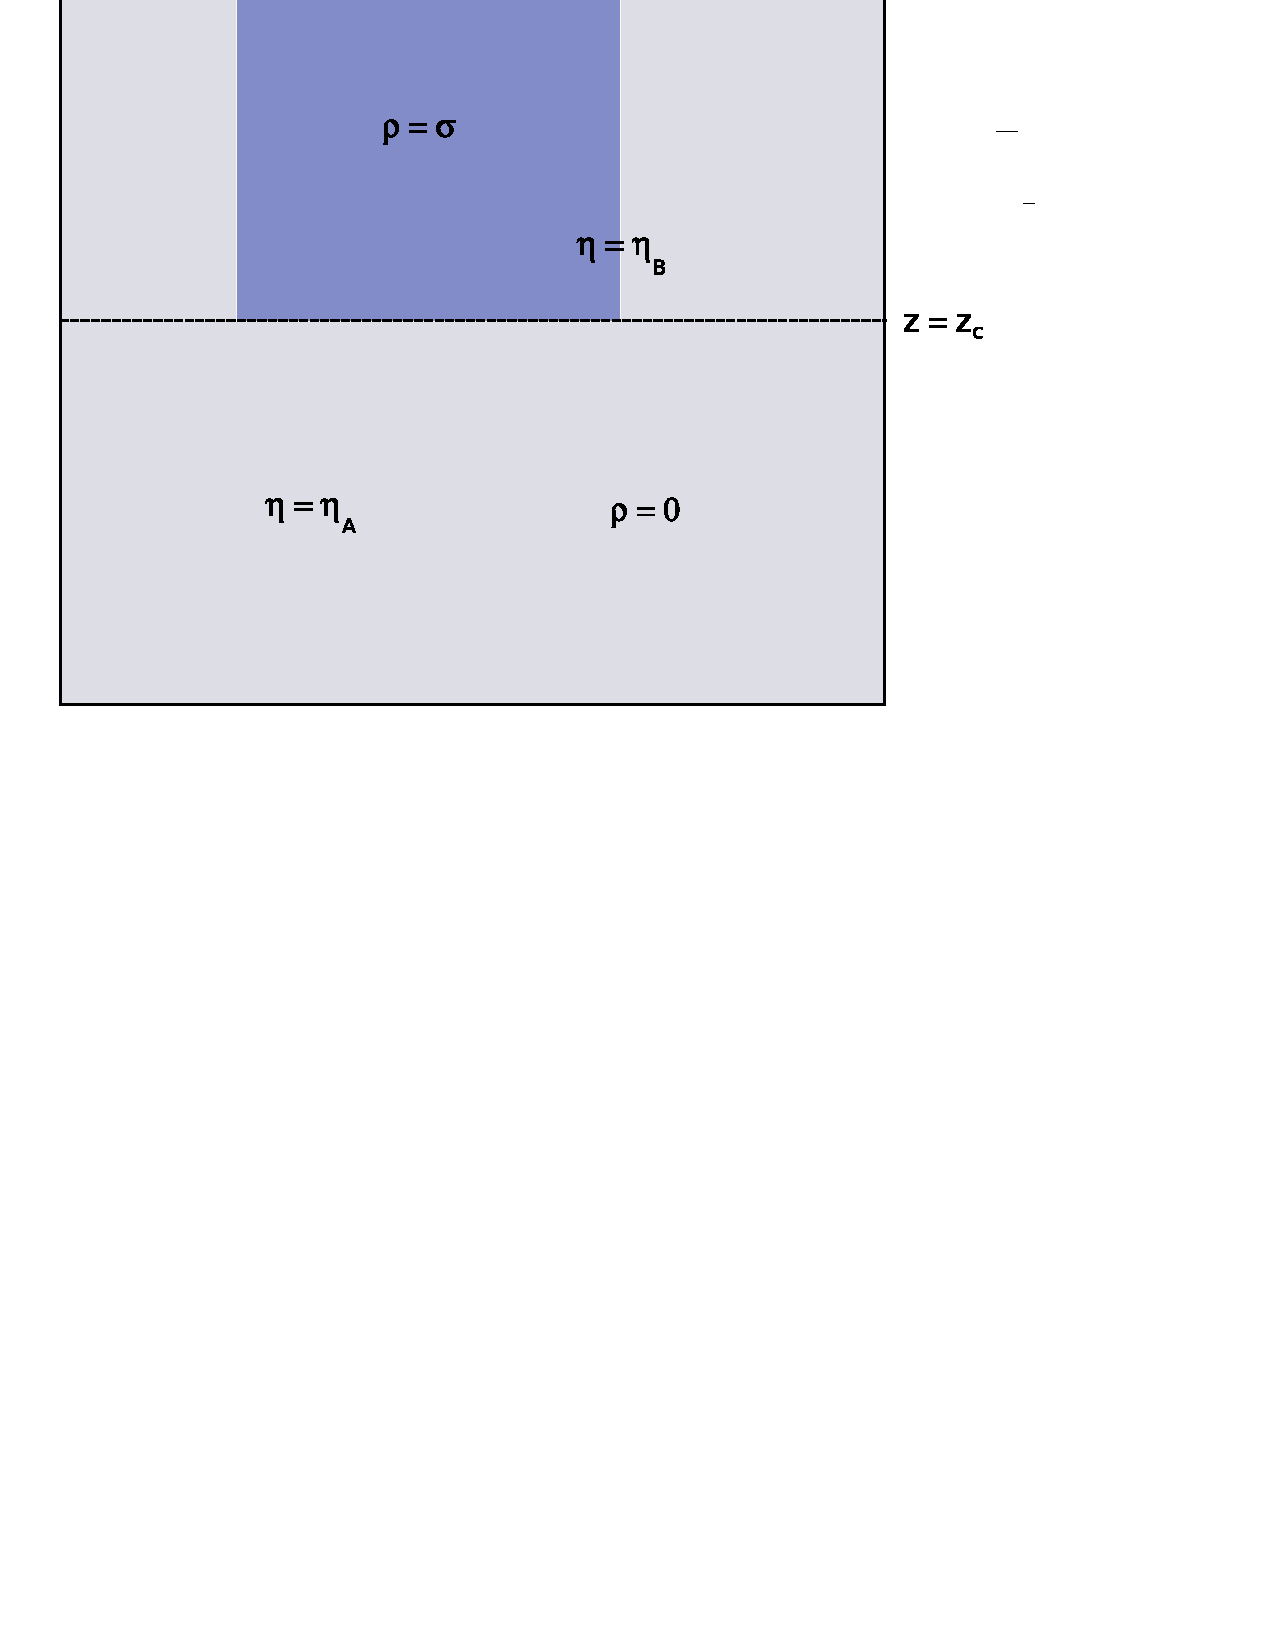
\includegraphics[width=6cm,clip]{../figs/figG}
    \caption[Short caption]{\label{figG} 
      Solution ({\bf SolG}):
      This solution has a block of density $\rho = \sigma$ from $x_0-dx/2 < x < x_0+dx/2$ above
      $ z= z_c$.
      The viscosity is layered with a jump at $ z=z_c $.
      The boundary conditions are free slip everywhere on the surfaces of the unit box.}
  \end{SCfigure} 
  

